\documentclass{article}
\usepackage{graphicx} % Required for inserting images
\usepackage[polish]{babel}
\usepackage{hyperref}
\usepackage[T1]{fontenc}
\usepackage{float}
\usepackage{listings}

\title{Dokumentacja - Winda}
\author{Filip Jędrzejewski}
\date{2 Czerwca 2024}

\begin{document}

\maketitle

\section{Opis modelowanego systemu}

Winda to system transportu pionowego, który głównie umożliwia przemieszczanie się osób między różnymi poziomami budynku. Działanie windy opiera się na kilku kluczowych elementach:

\begin{enumerate}
    \item \textbf{Panel przycisków:} Pasażerowie wybierają piętro docelowe, naciskając odpowiedni przycisk na panelu (w windzie lub poza nią - przyciski na poszczególnych piętrach).
    \item \textbf{Sterowanie:} Sygnały z przycisków są przekazywane do sterownika windy, który analizuje żądania i podejmuje decyzje dotyczące ruchu kabiny.
    \item \textbf{Silnik:} Silnik elektryczny porusza kabiną windy w odpowiednim kierunku.
    \item \textbf{Kabina:} Kabina windy porusza się w szybie windowym przewożąc pasażerów.
    \item \textbf{Drzwi:} Drzwi kabiny i drzwi zewnętrzne (piętra) otwierają się i zamykają automatycznie, umożliwiając bezpieczne wejście i wyjście pasażerów.
    \item \textbf{Wyświetlacz:} Wyświetlacz informuje pasażerów o aktualnym położeniu kabiny.
\end{enumerate}

Cykl działania przykładowej windy:

\begin{enumerate}
    \item Pasażer naciska przycisk, wskazując piętro docelowe.
    \item Sterownik windy odbiera sygnał i analizuje go, uwzględniając aktualne położenie kabiny i inne żądania.
    \item Sterownik wysyła polecenie do silnika, aby rozpocząć ruch w odpowiednim kierunku.
    \item Silnik napędza kabinę poruszającą się w szybie windowym.
    \item Gdy kabina osiągnie żądane piętro, sterownik wysyła polecenie do silnika, aby zatrzymać windę.
    \item Sterownik wysyła polecenie do drzwi kabiny i drzwi piętra, aby się otworzyły.
    \item Pasażerowie wchodzą lub wychodzą z windy.
    \item Po określonym czasie lub po naciśnięciu przycisku zamknięcia drzwi, sterownik wysyła polecenie zamknięcia drzwi.
    \item Po zamknięciu drzwi, winda jest gotowa do przyjęcia kolejnego żądania (cykl się powtarza).
\end{enumerate}


\section{Rozwiązanie}

\subsection{Schemat rozwiązania}

W celu rozwiązania zadania stworzono następujący diagram \texttt{Orange}:


\begin{figure}[H]
    \centering
    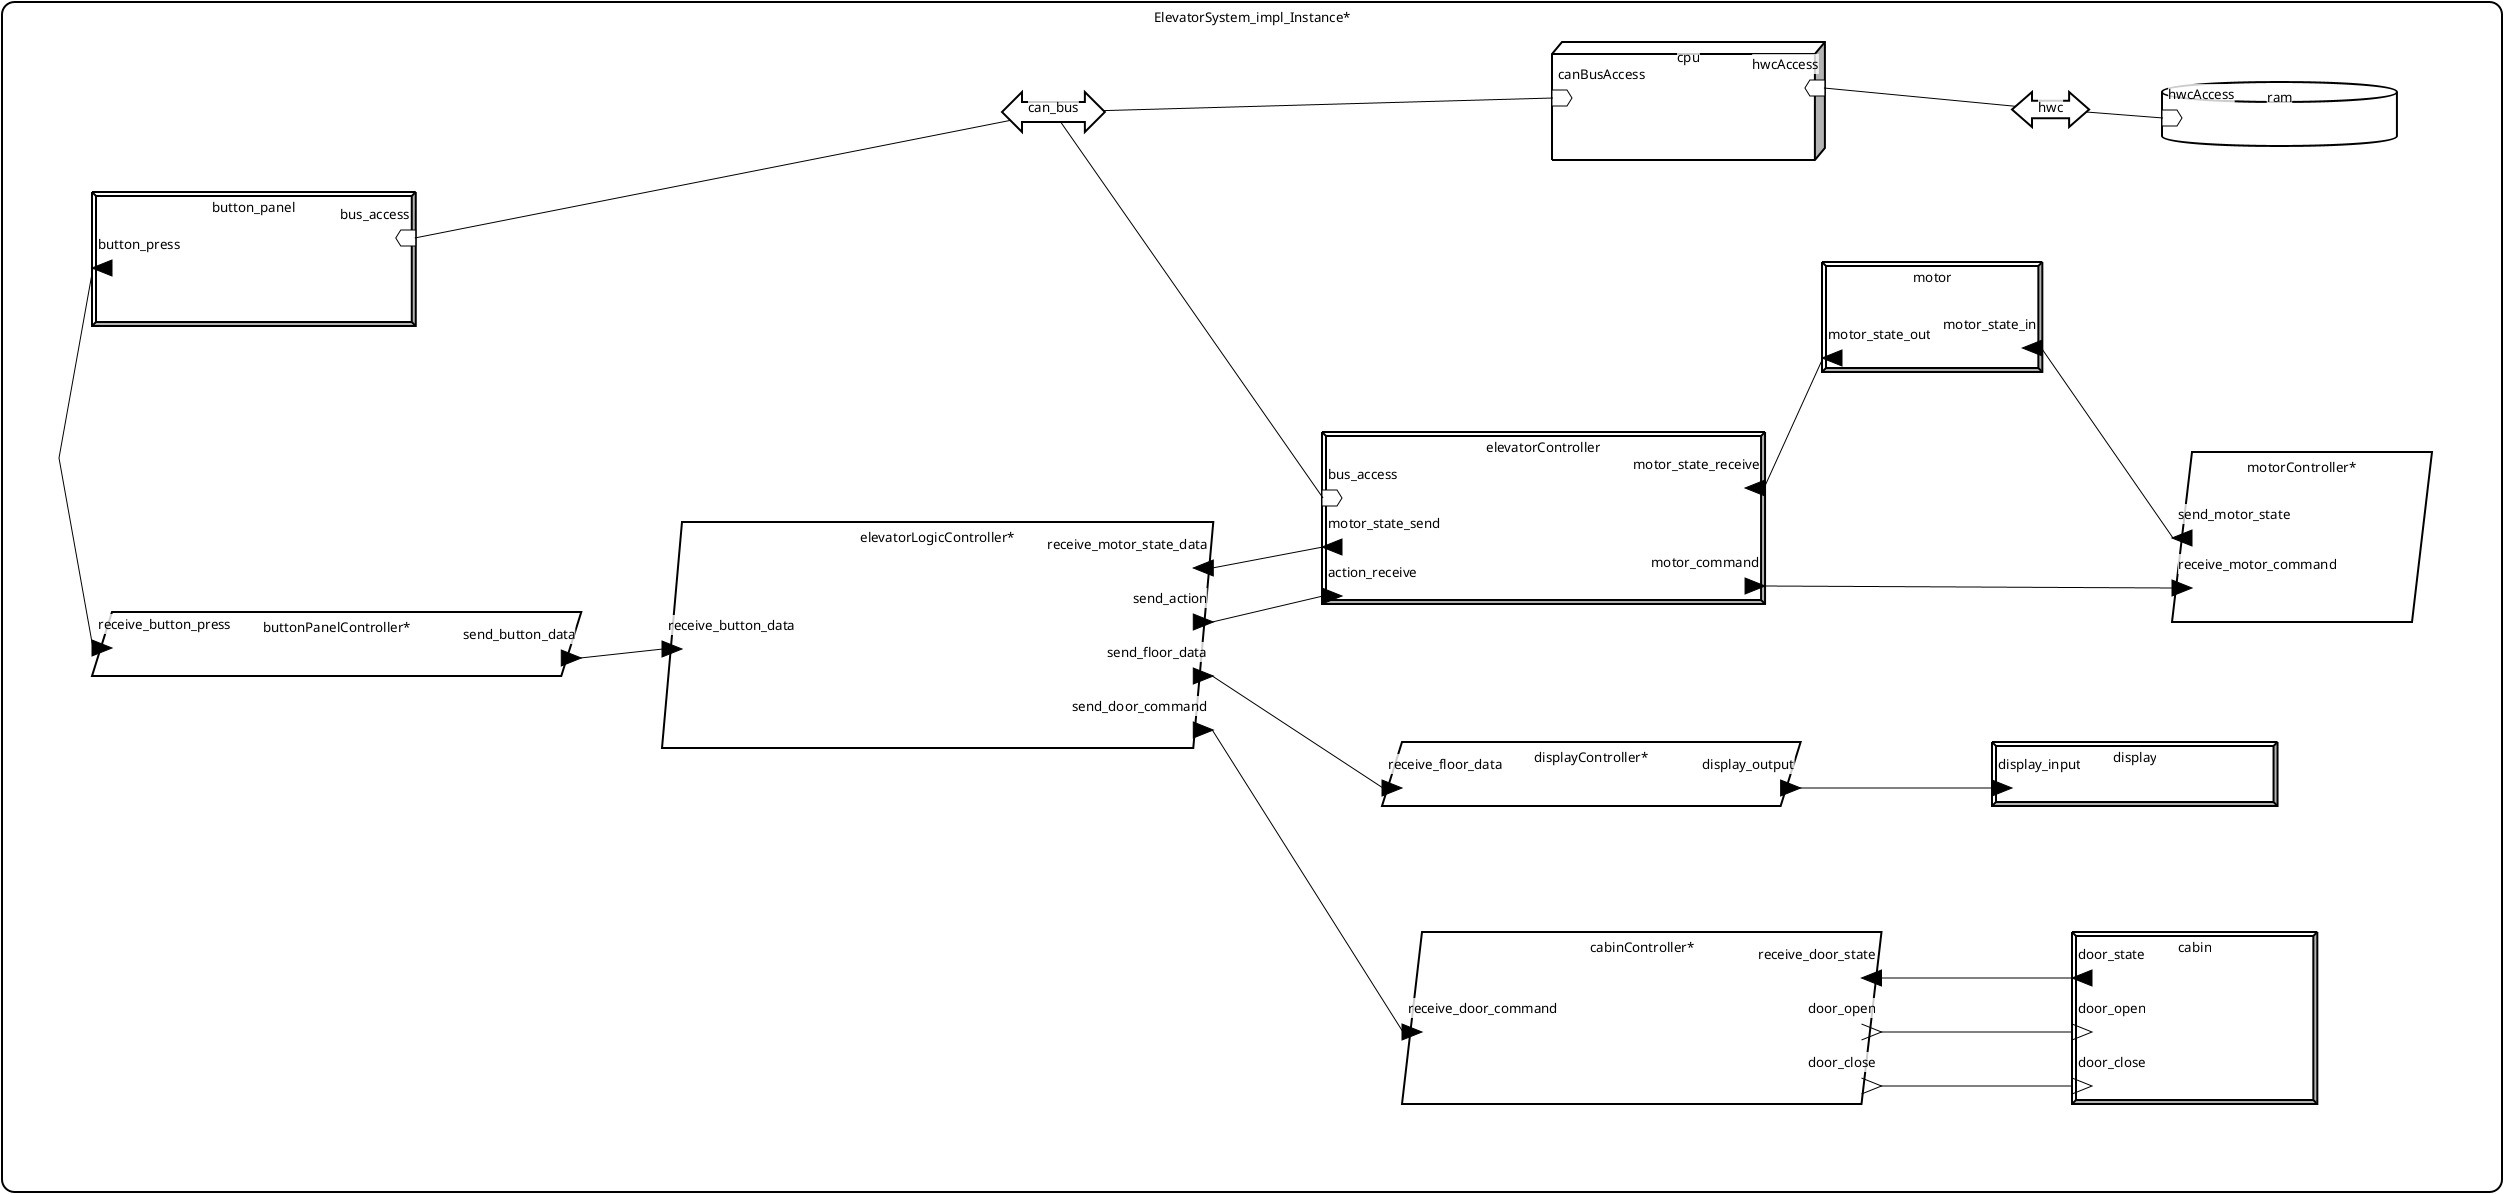
\includegraphics[width=1.2\linewidth]{./images/schema.png}
\end{figure}













\end{document}